\documentclass[aspectratio=169]{beamer}

\usepackage[utf8]{inputenc}
\mode<presentation>
\usetheme[visual,slim,framecount]{tptng}

\usepackage[T1]{fontenc}
\graphicspath{{../../dataset/figs/}{images/}{pdfs/}{figs/}}
\DeclareGraphicsExtensions{.pdf,.png,.jpg}

\usepackage[french]{babel}
\usepackage[babel]{microtype}
\usepackage{booktabs}
\usepackage{tikz}
\usetikzlibrary{positioning}
\usepackage{xcolor}

\AtBeginSection[]{
  \contentsframe[currentsection]
}
\renewcommand*{\contentsframename}{Plan}

%------------------------------------------------------------------------------
\title{BTGenBot $\times$ NAV4RAIL}
\subtitle{Semaine 1 --- EDA et préparation du dataset}

\author{Benjamin Lepourtois \and Anne Faury \and Mohamed Amar \and Mourad Latoundji}
\institute{Télécom Paris}
\date[28 mai 2026]{28 mai 2026 \\ {\small Mastère spécialisé IA/DATA --- Promotion 2026}}
%------------------------------------------------------------------------------

\begin{document}

\maketitle

%------------------------------------------------------------------------------
\section{Plan de travail et posture}
%------------------------------------------------------------------------------

\begin{frame}
  \frametitle{Rappel --- plan semaine 1 (cf. kickoff)}

  \begin{columns}[T]
    \begin{column}{0.55\textwidth}
      \textbf{Objectifs annoncés :}
      \begin{itemize}\itemsep2pt
        \item Téléchargement dataset BTGenBot
        \item EDA : catégories, longueur BTs, vocabulaire nœuds
        \item Conversion JSONL + adaptation prompt
      \end{itemize}

      \vspace{0.5em}
      \textbf{Livrable concret :}
      \begin{itemize}\itemsep2pt
        \item 1 notebook synthèse unifié
        \item Dataset SFT-ready
        \item Rapports MD + figures réutilisables
      \end{itemize}
    \end{column}
    \begin{column}{0.45\textwidth}
      \begin{alertblock}{Posture méthodologique}
        \small \textbf{Fidélité maximale au papier} BTGenBot (Izzo 2024).

        \vspace{0.3em}
        Le papier ne mentionne aucun filtrage, le repo officiel ne livre pas le script d'entraînement.

        \vspace{0.3em}
        On garde les \textbf{594 exemples bruts}, on documente tout le reste.
      \end{alertblock}
    \end{column}
  \end{columns}
\end{frame}

%------------------------------------------------------------------------------
\section{Dataset et chiffres clés}
%------------------------------------------------------------------------------

\begin{frame}
  \frametitle{Dataset BTGenBot --- état initial}

  \begin{columns}[T]
    \begin{column}{0.55\textwidth}
      \textbf{Source :}
      \begin{itemize}\itemsep2pt
        \item Dépôt officiel \href{https://github.com/AIRLab-POLIMI/BTGenBot}{\texttt{AIRLab-POLIMI/BTGenBot}}
        \item \texttt{dataset/bt\_dataset.json}, 2.2 MB
        \item Diff byte-à-byte vs fichier local $\to$ identique
      \end{itemize}

      \vspace{0.5em}
      \textbf{Format :} Alpaca
      \begin{itemize}\itemsep2pt
        \item \texttt{instruction} (consigne système)
        \item \texttt{input} (description NL de la tâche)
        \item \texttt{output} (Behavior Tree en XML)
      \end{itemize}

      \vspace{0.5em}
      \textbf{Volume :} \textbf{594} paires (papier annonce $\sim$600)
    \end{column}
    \begin{column}{0.42\textwidth}
      \begin{exampleblock}{Origine des BTs}
        \small Behavior Trees extraits de projets ROS2 open-source (Nav2, ROBORTS, etc.).

        \vspace{0.3em}
        Descriptions NL générées par GPT-3.5-turbo à partir des BTs.

        \vspace{0.3em}
        $\Rightarrow$ Dataset \textbf{semi-synthétique}.
      \end{exampleblock}
    \end{column}
  \end{columns}
\end{frame}

\begin{frame}
  \frametitle{Chiffres clés consolidés}

  \begin{columns}[T]
    \begin{column}{0.50\textwidth}
      {\scriptsize\begin{tabular}{lr}
        \toprule
        \textbf{Métrique} & \textbf{Valeur} \\
        \midrule
        Total exemples & 594 \\
        XML valides (parse strict) & 578 (97.31\%) \\
        XML valides (cleaning étendu) & 571 (96.13\%) \\
        \midrule
        Longueur input (mots), médiane & 117 \\
        Longueur input (mots), p95 & 158 \\
        \midrule
        Longueur XML (chars), médiane & 1 080 \\
        Longueur XML (chars), p95 & 11 878 \\
        Longueur XML (chars), max & 31 681 \\
        \midrule
        Nb nœuds BT, médiane / max & 15 / 399 \\
        Profondeur BT, médiane / max & 5 / 21 \\
        \midrule
        Tags XML uniques & 360 \\
        Skills métier uniques & \textbf{1 223} \\
        Variables blackboard \texttt{\{var\}} uniques & 296 \\
        \bottomrule
      \end{tabular}}
    \end{column}
    \begin{column}{0.48\textwidth}
      \begin{exampleblock}{Lecture}
        \small
        \begin{itemize}\itemsep1pt
          \item Inputs \textbf{très homogènes} (médiane 117 mots, p95 158)
          \item XML \textbf{très asymétrique} : médiane 1k chars, max 31k
          \item Arbres variés : 15 nœuds typique, jusqu'à 399 (Nav2 cascadé)
          \item \textbf{1\,223 skills uniques} = vocabulaire ouvert (vs catalogue fermé SNCF, 28 skills)
        \end{itemize}
      \end{exampleblock}
    \end{column}
  \end{columns}
\end{frame}

\begin{frame}
  \frametitle{Longueurs : input vs output XML}

  \begin{center}
    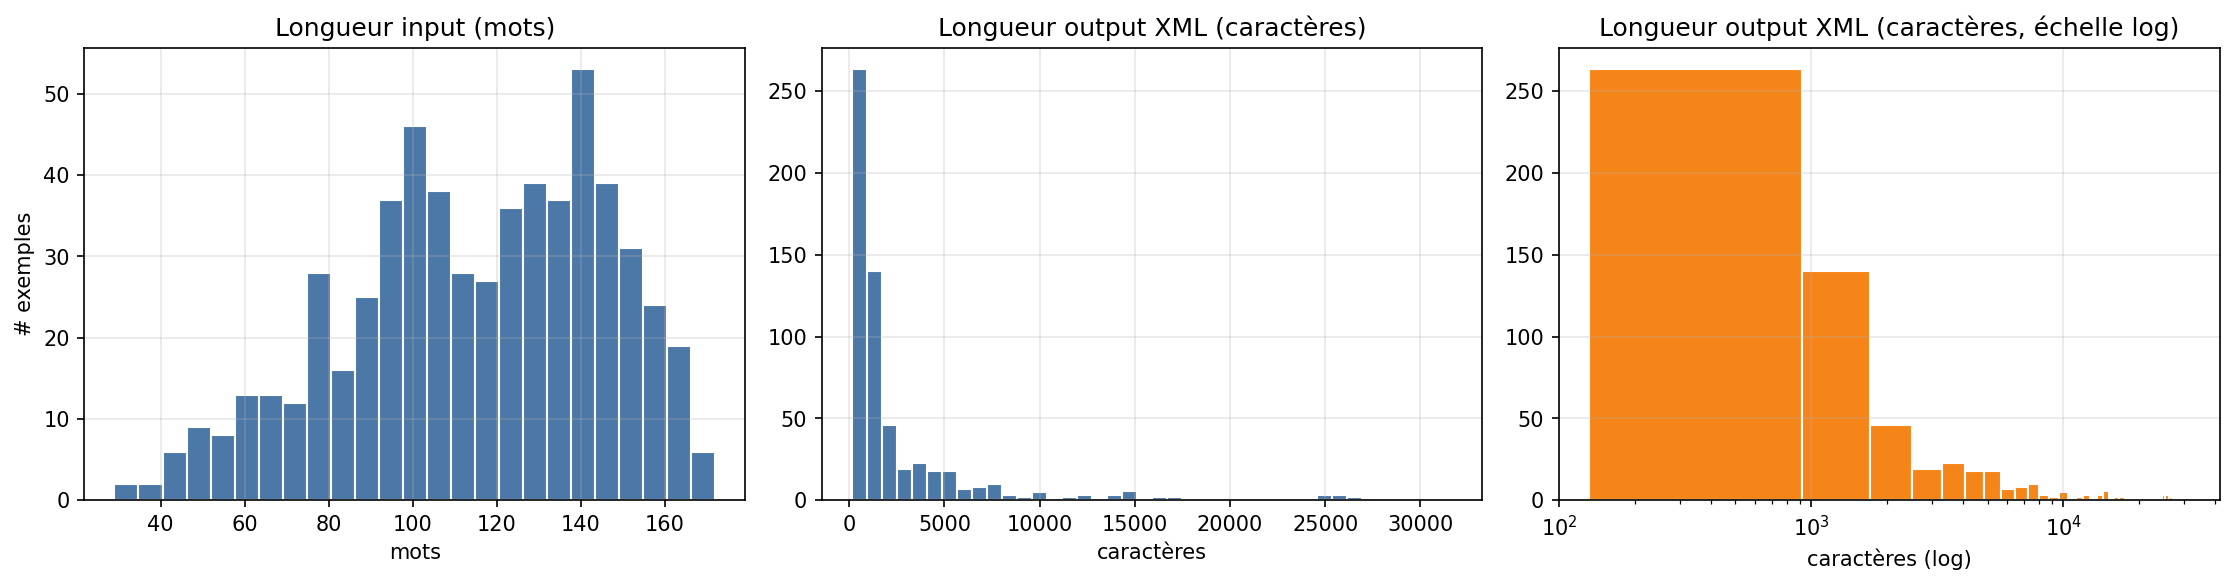
\includegraphics[width=0.95\textwidth]{longueurs.png}
  \end{center}

  \vspace{-0.5em}
  {\small
  Input : distribution \textbf{gaussienne resserrée} (prompt court généré uniformément par GPT-3.5).
  Output : distribution \textbf{log-normale} avec longue traîne --- quelques BTs Nav2 monstrueux dominent les statistiques.}
\end{frame}

\begin{frame}
  \frametitle{Vocabulaire XML --- structure vs domaine}

  \begin{columns}[T]
    \begin{column}{0.50\textwidth}
      \begin{center}
        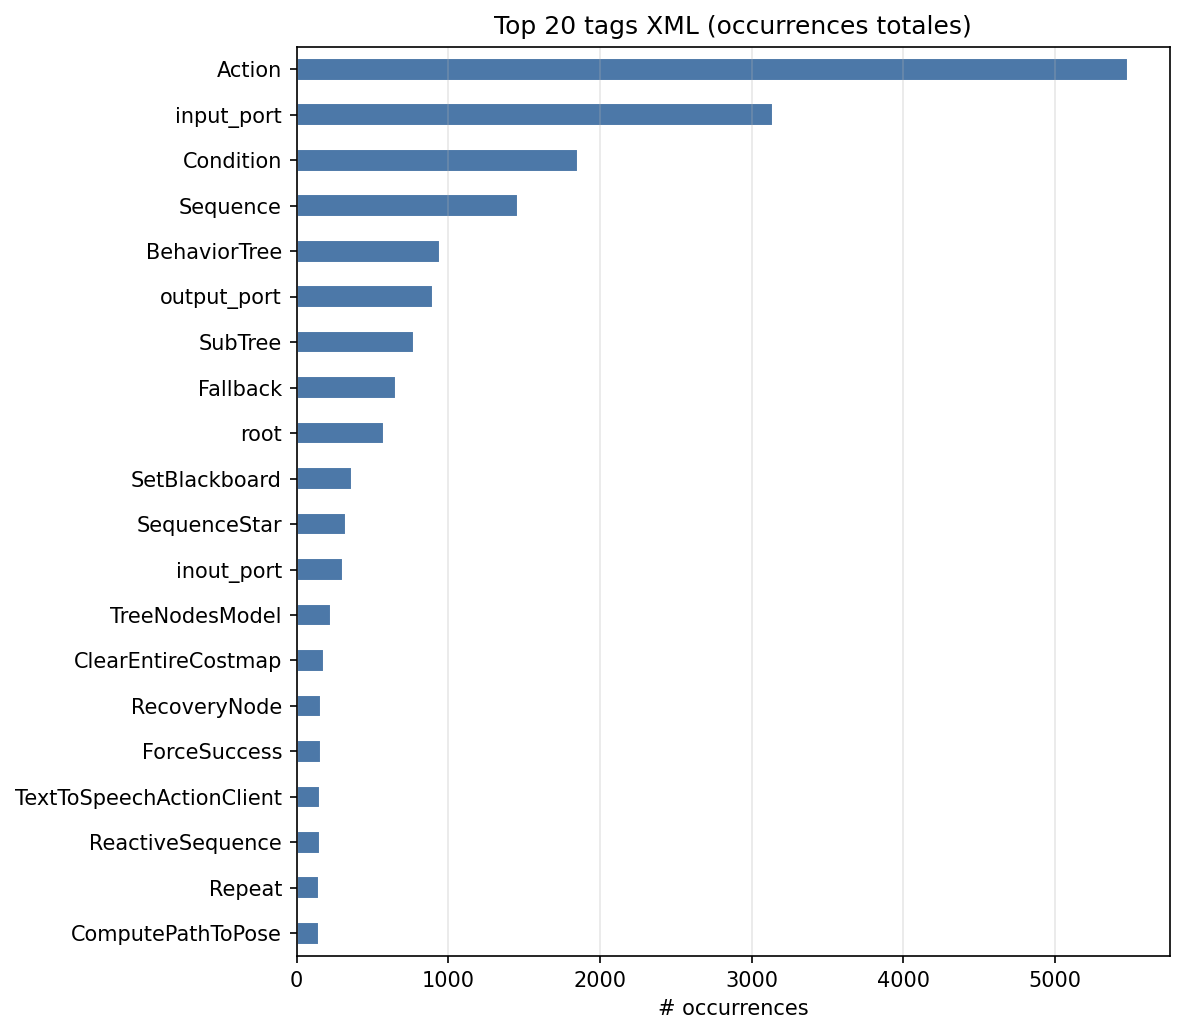
\includegraphics[width=\textwidth]{top_tags.png}
      \end{center}
    \end{column}
    \begin{column}{0.48\textwidth}
      {\scriptsize\begin{tabular}{lr}
        \toprule
        Couche & Volume \\
        \midrule
        Tags XML uniques (total) & 360 \\
        Nœuds de contrôle BT.CPP & $\sim$12 \\
        Skills domaine uniques & \textbf{1 223} \\
        Variables blackboard \texttt{\{var\}} & 296 \\
        \midrule
        \multicolumn{2}{l}{\textit{Occurrences dans le dataset :}} \\
        \texttt{Action} & 2 605 \\
        \texttt{Sequence} & 855 \\
        \texttt{SubTree} & 622 \\
        \texttt{Fallback} & 299 \\
        \bottomrule
      \end{tabular}}

      \vspace{0.5em}
      \begin{exampleblock}{Deux niveaux d'abstraction}
        \small Syntaxe structurelle (12 nœuds, stable) \textbf{+} vocabulaire ouvert (1\,223 skills, domaine-dépendant).
        Le modèle doit apprendre les deux simultanément.
      \end{exampleblock}
    \end{column}
  \end{columns}
\end{frame}

\begin{frame}
  \frametitle{Complexité structurelle par catégorie}

  \begin{columns}[T]
    \begin{column}{0.55\textwidth}
      \begin{center}
        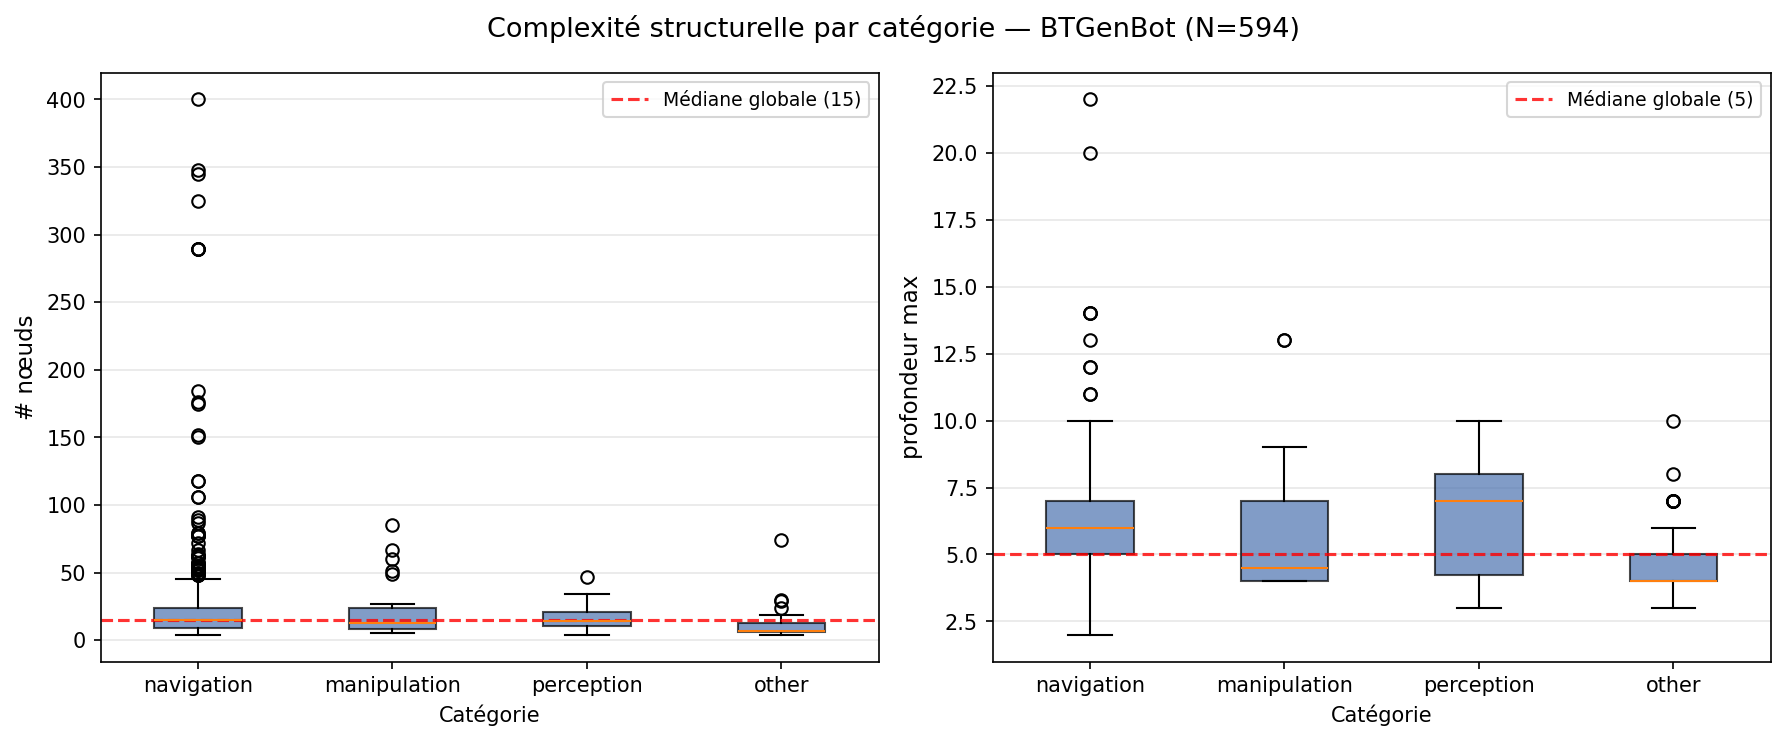
\includegraphics[width=\textwidth]{complexity_by_category.png}
      \end{center}
    \end{column}
    \begin{column}{0.43\textwidth}
      {\scriptsize\begin{tabular}{lrr}
        \toprule
        Catégorie & Nœuds & Prof. \\
        \midrule
        navigation (N=434) & 14 & 6 \\
        \quad + recovery (192) & 22 & 7 \\
        manipulation (N=43) & 12 & 5 \\
        perception (N=15) & 13 & 7 \\
        other (N=100) & 6 & 4 \\
        \midrule
        \textit{NAV4RAIL réel} & \textit{112} & \textit{$\sim$7} \\
        \bottomrule
      \end{tabular}}

      \vspace{0.4em}
      {\scriptsize
      Perception : profondeur = navigation+recovery avec \textbf{15$\times$ moins d'exemples} --- variance élevée.

      \vspace{0.3em}
      NAV4RAIL réel hors-échelle : 7$\times$ plus grand que la médiane dataset.}
    \end{column}
  \end{columns}
\end{frame}

%------------------------------------------------------------------------------
\section{Validité XML et structure}
%------------------------------------------------------------------------------

\begin{frame}
  \frametitle{Validité XML --- 16 exemples non parsables}

  \begin{columns}[T]
    \begin{column}{0.48\textwidth}
      \textbf{Distribution des erreurs :}

      \vspace{0.3em}
      {\scriptsize\begin{tabular}{p{4.5cm}r}
        \toprule
        Type d'erreur & Count \\
        \midrule
        Token invalide (commentaires \texttt{<!---->} malformés, attributs sans guillemets) & 12 \\
        Tag non fermé / mal fermé & 4 \\
        \midrule
        \textbf{Total invalides} & \textbf{16} (2.7\%) \\
        \bottomrule
      \end{tabular}}

      \vspace{0.6em}
      \textbf{Origine :} bugs de génération GPT-3.5 --- XML « presque valide ». Cohérent avec dataset semi-synthétique.
    \end{column}
    \begin{column}{0.50\textwidth}
      \begin{alertblock}{Décision}
        \small \textbf{Dataset conservé à 594 entiers.}

        \vspace{0.3em}
        Le papier ne filtre pas. \texttt{SFTTrainer} apprend du texte, ne valide pas le XML. Les 16 invalides (2.7\%) seront appris comme texte ordinaire --- bruit négligeable.

        \vspace{0.3em}
        On documente, on filtre pas.
      \end{alertblock}
    \end{column}
  \end{columns}
\end{frame}

\begin{frame}
  \frametitle{Structure des Behavior Trees}

  \begin{center}
    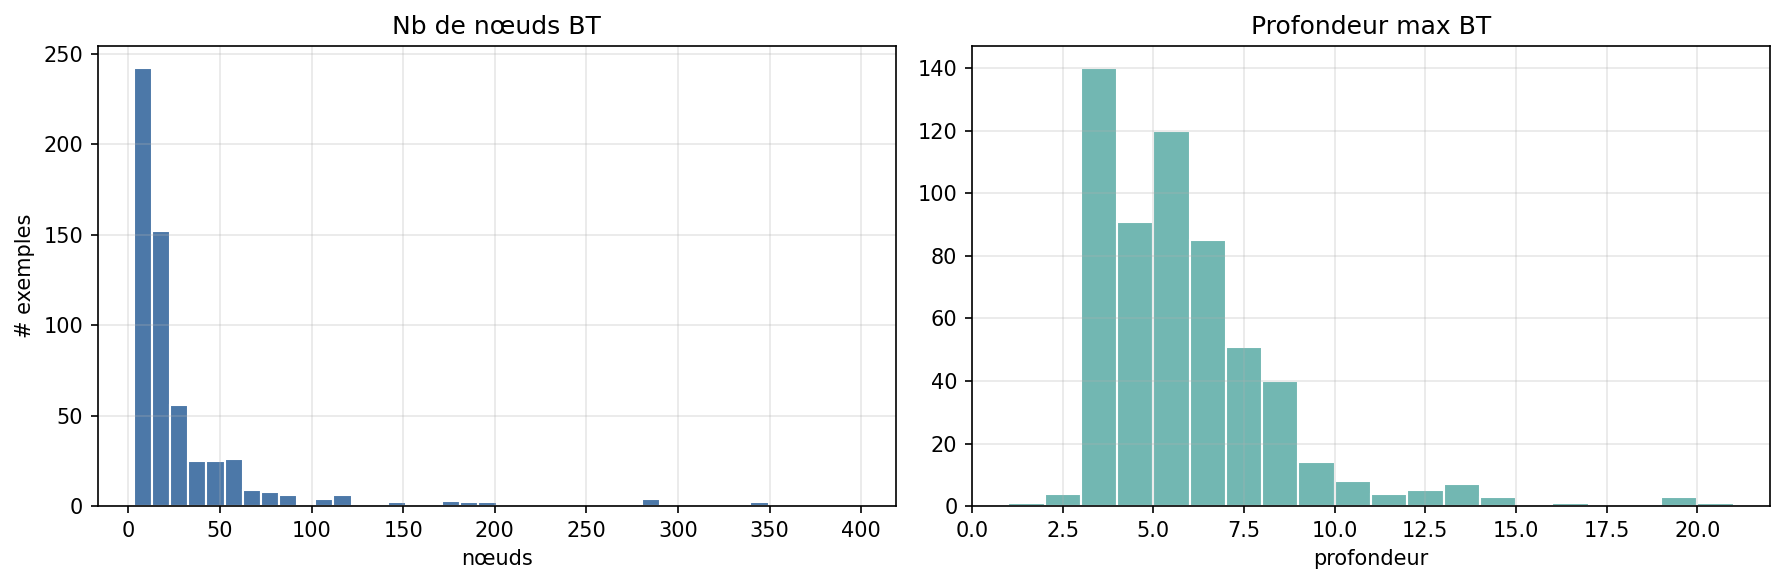
\includegraphics[width=0.85\textwidth]{structure.png}
  \end{center}

  \vspace{-0.4em}
  \begin{center}
  {\small
  La plupart des BTs sont \textbf{petits à moyens} (médiane 15 nœuds, profondeur 5) mais quelques arbres atteignent 399 nœuds et 21 niveaux --- scénarios Nav2 complets avec recovery cascadé.}
  \end{center}
\end{frame}

\begin{frame}
  \frametitle{Métriques de complexité --- distribution par catégorie}

  \begin{center}
    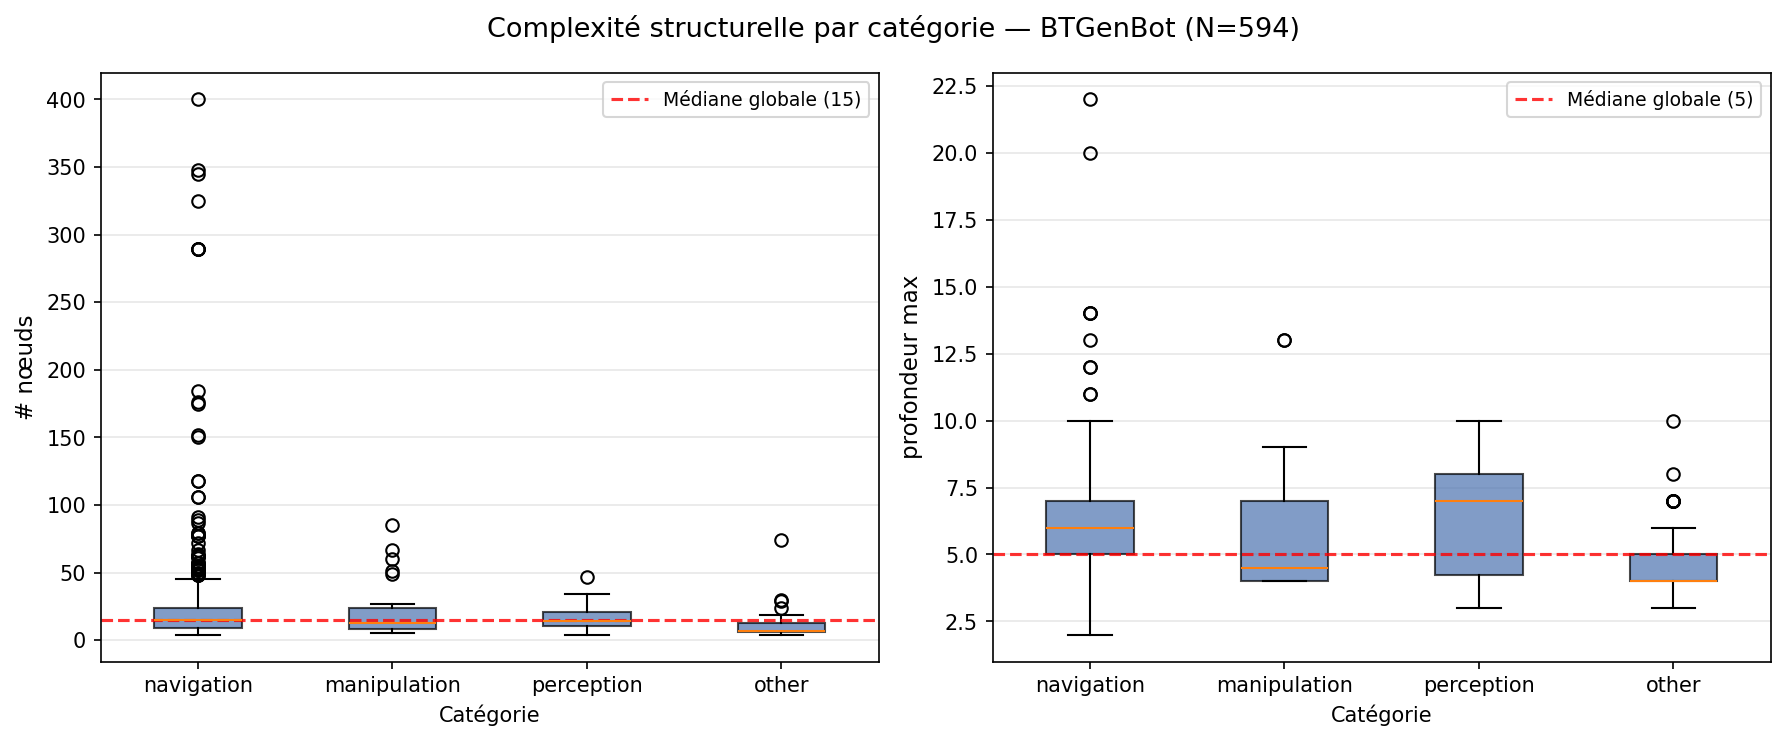
\includegraphics[width=0.90\textwidth]{complexity_by_category.png}
  \end{center}

  \vspace{-0.4em}
  \begin{center}
  {\scriptsize
  Navigation avec recovery : médiane \textbf{22 nœuds}, profondeur \textbf{7} --- 60\% plus complexe que navigation simple.
  Perception : profondeur élevée (7) sur seulement \textbf{15 exemples} --- variance forte, signal faible.
  Ligne rouge = médiane globale du dataset. Le BT NAV4RAIL réel (112 nœuds) est hors-échelle.}
  \end{center}
\end{frame}

\begin{frame}
  \frametitle{Largeur des BTs --- profil par niveau de profondeur}

  \begin{center}
    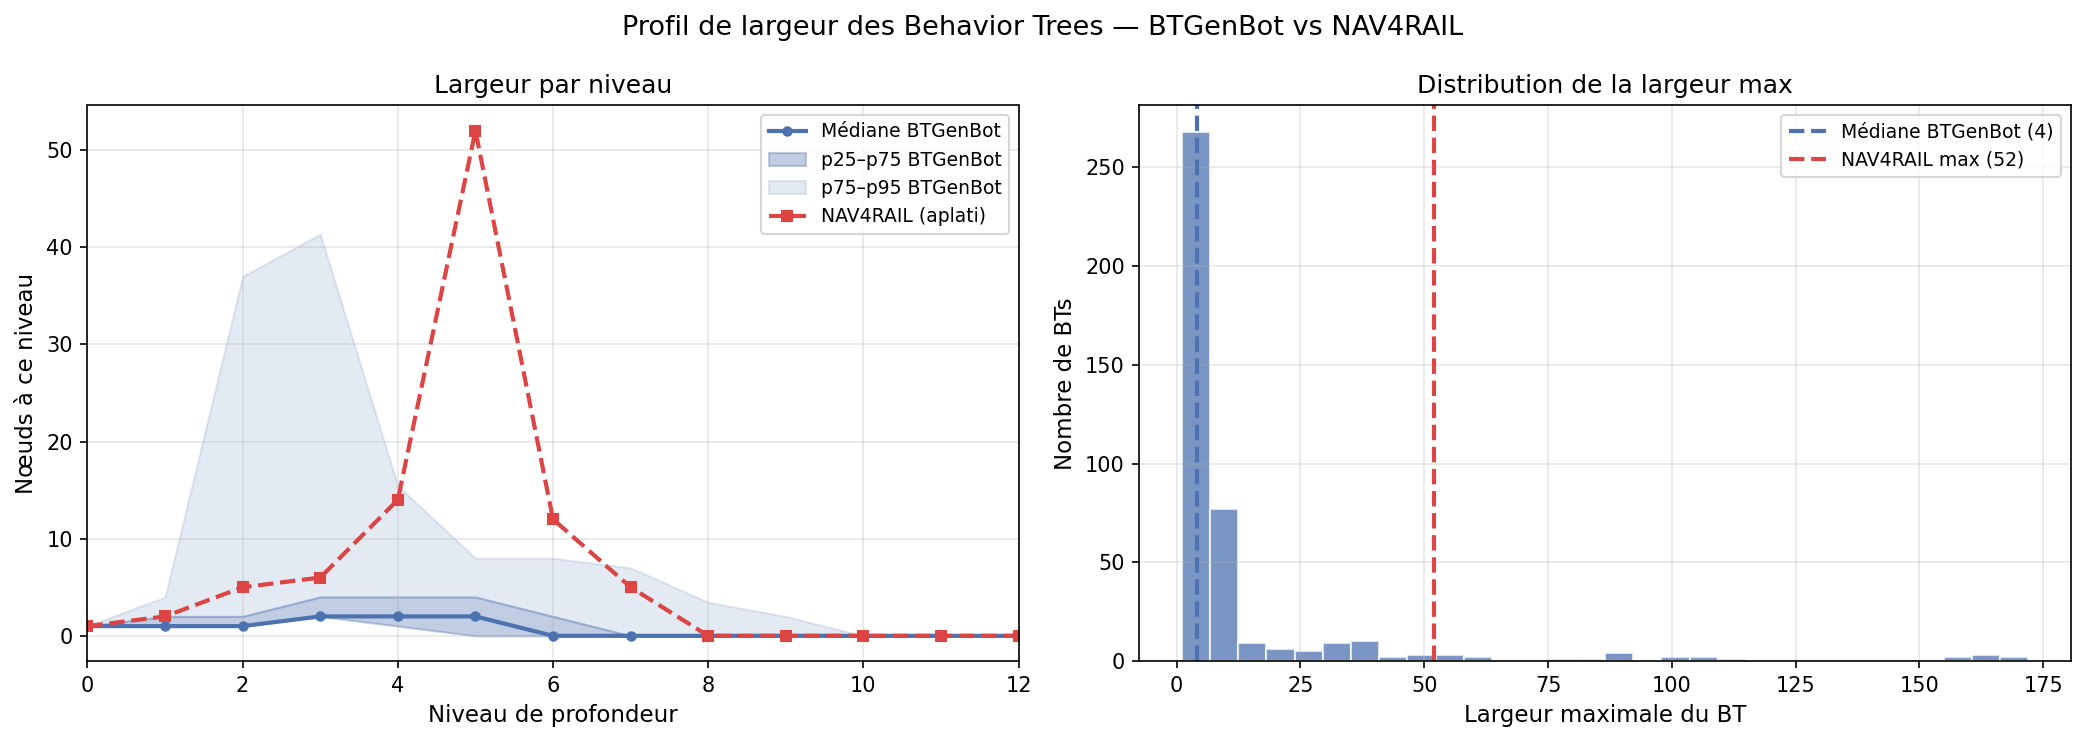
\includegraphics[width=0.90\textwidth]{width_profile.png}
  \end{center}

  \vspace{-0.3em}
  \begin{center}
  {\scriptsize
  \textbf{BTGenBot :} largeur médiane max = \textbf{4} nœuds (p95 = 55). Distribution très resserrée : la majorité des BTs restent étroits.
  \textbf{Exemple NAV4RAIL :} pic à profondeur 5 avec \textbf{52 nœuds} (9 primitives de mouvement $\times$ actions imbriquées) --- \textbf{13$\times$ plus large} que la médiane dataset.

  $\Rightarrow$ Le modèle entraîné ne génère jamais de BTs aussi larges : risque de génération de structures linéaires (une branche unique) pour des tâches multi-primitives.}
  \end{center}
\end{frame}

\begin{frame}
  \frametitle{SubTreePlus --- absent du dataset, central dans NAV4RAIL}

  \begin{columns}[T]
    \begin{column}{0.50\textwidth}
      \textbf{Dans BTGenBot (594 BTs) :}

      \vspace{0.4em}
      {\scriptsize\begin{tabular}{lr}
        \toprule
        Tag & Occurrences \\
        \midrule
        \texttt{SubTree} (API v3) & 622 (dans 90 BTs, 15\%) \\
        \texttt{SubTreePlus} (API v4) & \textbf{0} \\
        \bottomrule
      \end{tabular}}

      \vspace{0.6em}
      \textbf{Dans NAV4RAIL réel :}

      \vspace{0.4em}
      {\scriptsize\begin{tabular}{lr}
        \toprule
        Tag & Occurrences \\
        \midrule
        \texttt{SubTreePlus} & \textbf{15} \\
        \multicolumn{2}{l}{Architecture entièrement modulaire} \\
        \multicolumn{2}{l}{\texttt{\_\_autoremap="true"} + remapping ports} \\
        \bottomrule
      \end{tabular}}
    \end{column}
    \begin{column}{0.48\textwidth}
      \begin{alertblock}{Conséquence pour la génération}
        \small Le modèle ne produira \textbf{jamais} \texttt{SubTreePlus} spontanément.

        \vspace{0.3em}
        Il générera soit :
        \begin{itemize}
          \item un arbre \textbf{monolithique} plat (distribution entraînement)
          \item du \texttt{SubTree} v3 (présent à 15\% en training)
        \end{itemize}

        \vspace{0.3em}
        $\Rightarrow$ Sans contrainte explicite dans le prompt, les BTs générés sont \textbf{structurellement incompatibles} avec l'architecture NAV4RAIL.
      \end{alertblock}
    \end{column}
  \end{columns}
\end{frame}

%------------------------------------------------------------------------------
\section{Catégorisation et recovery patterns}
%------------------------------------------------------------------------------

\begin{frame}
  \frametitle{Catégories descriptives --- méthode hybride}

  \begin{center}
    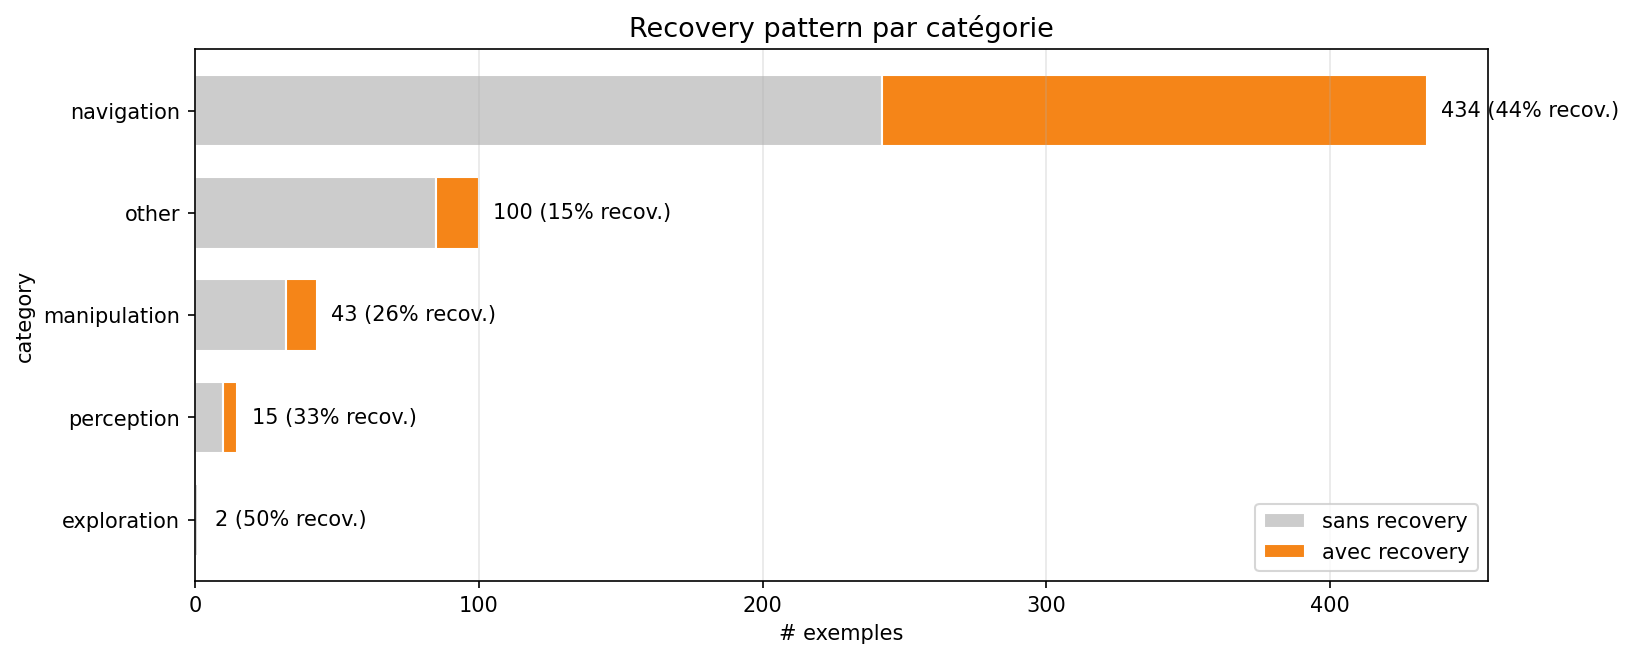
\includegraphics[width=0.92\textwidth]{categories_recovery.png}
  \end{center}

  \vspace{-0.3em}
  \begin{center}
  {\scriptsize
  \textbf{Méthode :} signal XML (skills présents) prioritaire, fallback regex sur input texte. 5 catégories canoniques.
  \textbf{Flag transverse} \texttt{has\_recovery\_pattern} = présence de \texttt{Fallback}/\texttt{RecoveryNode} avec \texttt{Sequence} imbriquée : \textbf{224 / 594} BTs (37.7\%), concentrés sur navigation (44\% des BTs nav).}
  \end{center}
\end{frame}

\begin{frame}
  \frametitle{Implication directe pour le transfert SNCF}

  \begin{columns}[T]
    \begin{column}{0.45\textwidth}
      \textbf{Distribution :}

      \vspace{0.3em}
      {\small\begin{tabular}{lr}
        \toprule
        Catégorie & \% \\
        \midrule
        \textbf{navigation} & \textbf{73.1\%} \\
        other & 16.8\% \\
        manipulation & 7.2\% \\
        \textbf{perception} & \textbf{2.5\%} \\
        exploration & 0.3\% \\
        \bottomrule
      \end{tabular}}
    \end{column}
    \begin{column}{0.52\textwidth}
      \begin{alertblock}{NAV4RAIL = navigation + perception}
        \small SNCF = inspection ferroviaire.

        \vspace{0.3em}
        Dataset BTGenBot \textbf{bien aligné navigation} (73\%) mais \textbf{faible perception} (15 exemples, 2.5\%).

        \vspace{0.3em}
        $\Rightarrow$ Mauvaise nouvelle pour le transfert direct sur les skills perception du catalogue SNCF.
      \end{alertblock}

      \vspace{0.3em}
      {\scriptsize Le modèle apprendra solidement les patterns Nav2 mais aura peu de signal pour la capture / analyse visuelle propres à l'inspection.}
    \end{column}
  \end{columns}
\end{frame}

\begin{frame}
  \frametitle{Anatomie comparative --- BTGenBot vs NAV4RAIL réel}

  \vspace{0.2em}
  \begin{center}
  {\scriptsize\begin{tabular}{p{2.8cm}p{4.3cm}p{4.3cm}}
    \toprule
    & \textbf{BTGenBot} (médiane dataset) & \textbf{NAV4RAIL réel} (\texttt{behavior\_tree\_example.xml}) \\
    \midrule
    Définitions BT        & 1                              & \textbf{16} (main + 15 sous-arbres) \\
    Nœuds totaux          & 15                             & \textbf{112} \\
    Profondeur max        & 5                              & $\sim$7 par sous-arbre \\
    Largeur max           & 4 (médiane)                    & \textbf{52} (exemple NAV4RAIL, profondeur 5) \\
    \texttt{SubTreePlus}  & 0                              & \textbf{15} \\
    Vocabulaire actions   & Nav2 (ClearEntireCostmap…)     & Inspection (ManageMeasurements…) \\
    Logique inspection    & absente                        & \textbf{centrale} \\
    \bottomrule
  \end{tabular}}
  \end{center}

  \vspace{0.3em}
  \begin{center}
  {\scriptsize $\Rightarrow$ NAV4RAIL \textbf{7$\times$ plus grand} (nœuds), largeur \textbf{13$\times$} plus large au pic (52 vs 4), entièrement modulaire via \texttt{SubTreePlus}, vocabulaire métier totalement distinct.}
  \end{center}
\end{frame}

\begin{frame}
  \frametitle{Bilan transférabilité --- ce qui passe, ce qui ne passe pas}

  \begin{center}
  {\scriptsize\begin{tabular}{p{2.2cm}p{5.0cm}p{4.5cm}}
    \toprule
    & Éléments & Justification \\
    \midrule
    \textbf{$\checkmark$ Transférable} &
      Nœuds de contrôle : \texttt{Sequence}, \texttt{Fallback}, \texttt{ReactiveFallback}, \texttt{Repeat} &
      Identiques BT.CPP 3.x et 4.x --- syntaxe partagée \\[0.3em]
    \textbf{$\sim$ Partiel} &
      Structure recovery \texttt{Fallback(Seq, Action)} &
      Motif présent (38\% des BTs) mais actions Nav2-spécifiques \\[0.3em]
    \textbf{$\times$ Non transférable} &
      Vocabulaire action/condition (0/43 skills NAV4RAIL dans training) ;
      \texttt{SubTreePlus} ; logique inspection &
      Jamais vu en training \\
    \bottomrule
  \end{tabular}}
  \end{center}

  \vspace{0.2em}
  \begin{center}
  \begin{minipage}{0.90\textwidth}
  \begin{alertblock}{Quelles pistes d'adaptation ?}
    \small Le modèle doit être guidé sur le vocabulaire et la structure NAV4RAIL.
    Mais comment ? \textbf{Prompt engineering} avec la liste des skills SNCF ?
    \textbf{Second SFT} sur quelques exemples NAV4RAIL ? \textbf{RAG} sur les spécifications des BTs cibles ?
    La réponse dépend du volume d'exemples disponibles --- aujourd'hui : \textbf{1 seul}.
  \end{alertblock}
  \end{minipage}
  \end{center}
\end{frame}

\begin{frame}
  \frametitle{Recovery patterns --- Top motifs Nav2}

  \begin{center}
    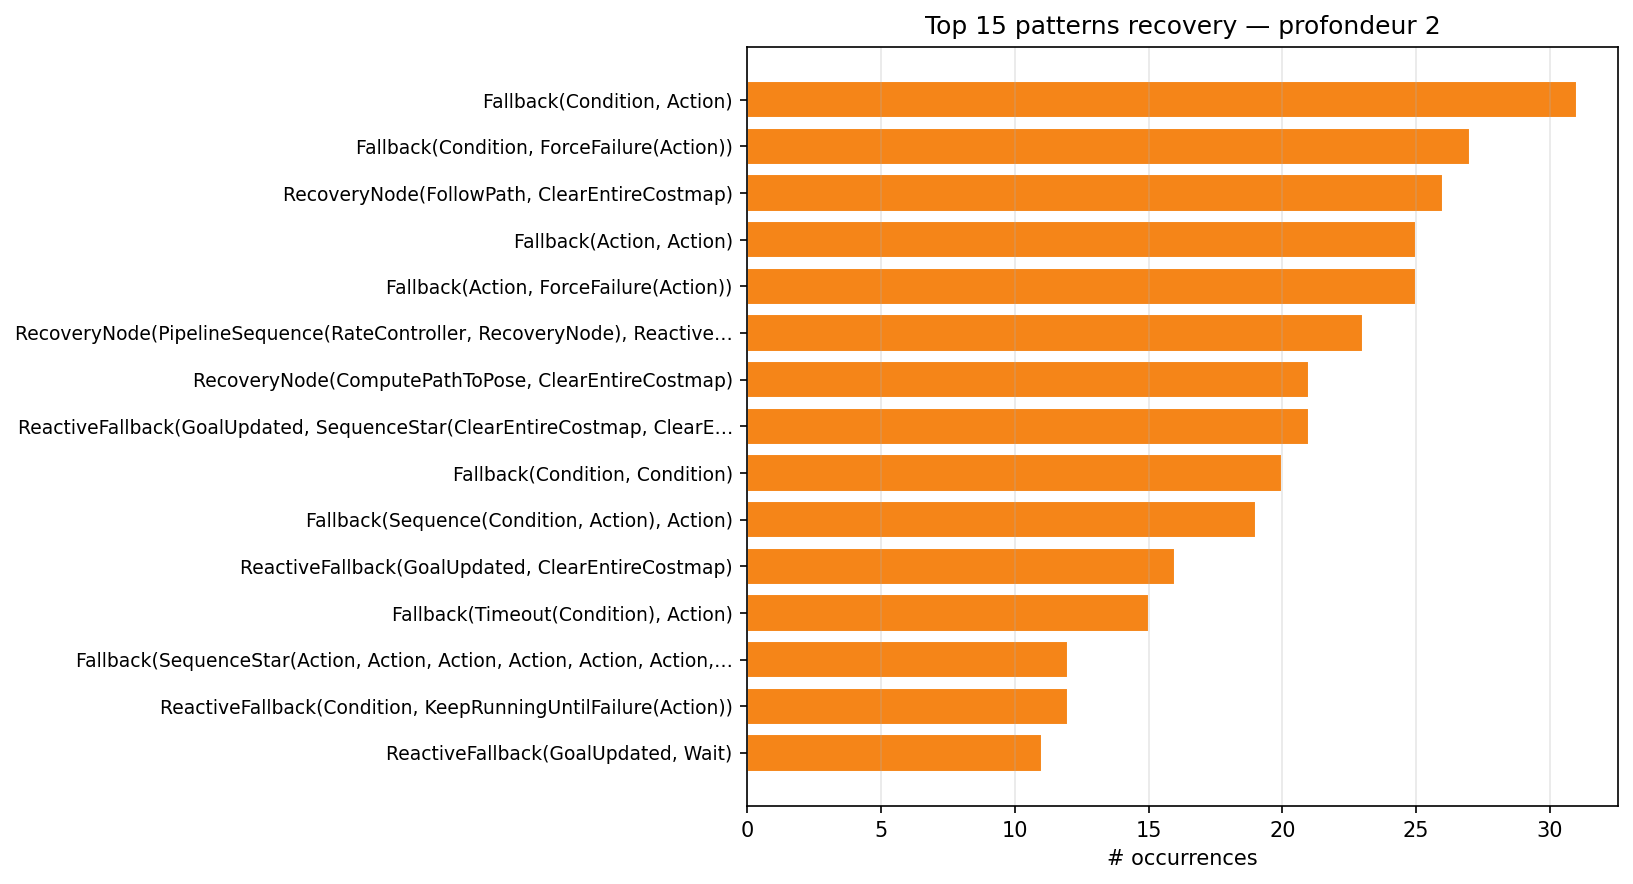
\includegraphics[width=0.70\textwidth]{recovery_patterns_d2.png}
  \end{center}

  \vspace{-0.3em}
  \begin{center}
  {\scriptsize
  \textbf{Top :} \texttt{Fallback(Condition, Action)} (31), \texttt{RecoveryNode(FollowPath, ClearEntireCostmap)} (26), \texttt{RecoveryNode(ComputePathToPose, ClearEntireCostmap)} (21).
  $\Rightarrow$ Signature canonique du recovery Nav2. Le modèle apprend la \textbf{syntaxe}, pas la sémantique. Ces patterns 2D ne sont pas transférables tels quels à NAV4RAIL : seule l'idée de séquence corrective reste pertinente.}
  \end{center}
\end{frame}

%------------------------------------------------------------------------------
\section{Token count}
%------------------------------------------------------------------------------

\begin{frame}
  \frametitle{Tokenization --- diagnostic critique vs papier}

  \begin{center}
    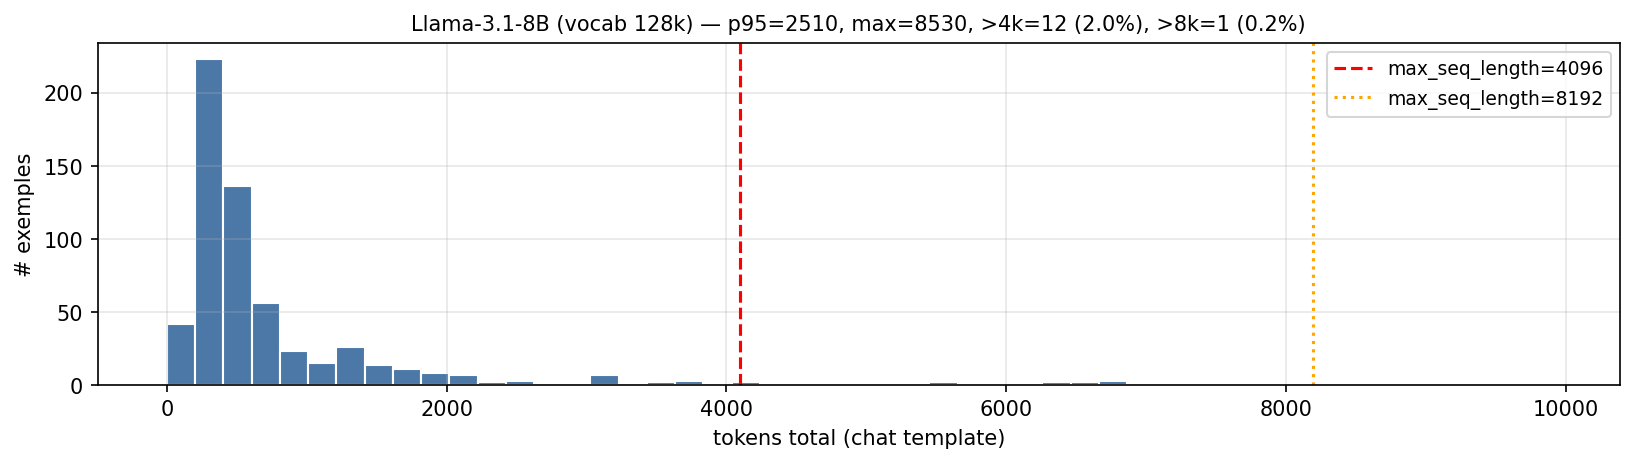
\includegraphics[width=0.78\textwidth]{tokens_distribution_llama.png} \\
    \vspace{0.2em}
    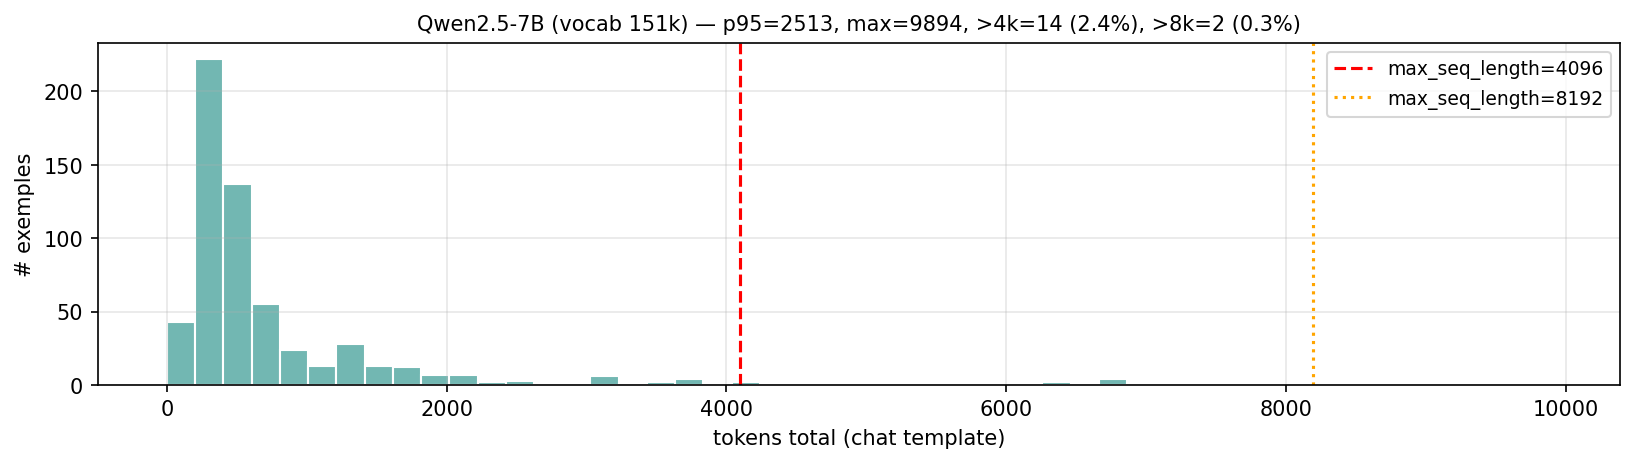
\includegraphics[width=0.78\textwidth]{tokens_distribution_qwen.png}
  \end{center}

  \vspace{-0.4em}
  {\scriptsize
  Papier fixe \texttt{max\_seq\_length=4096} sans documenter la distribution. \textbf{Notre mesure :} Llama-3.1 et Qwen2.5 quasi-équivalents (ratio médian = 1.000). Troncature à 4096 : 2.0--2.4\%.
  $\Rightarrow$ On garde 4096 (fidélité), on documente le taux. Ablation 8192 si VRAM le permet en QLoRA.}
\end{frame}

%------------------------------------------------------------------------------
\section{Synthèse}
%------------------------------------------------------------------------------

\begin{frame}
  \frametitle{Synthèse --- semaine 1 cochée, semaine 2 débloquée}

  \begin{columns}[T]
    \begin{column}{0.50\textwidth}
      \textbf{\small Livrables produits :}

      {\scriptsize
      \begin{itemize}\itemsep1pt
        \item 1 notebook synthèse unifié (\texttt{eda\_BT\_synthesis\_Benjamin.ipynb})
        \item 2 JSONL trainables (chat + Alpaca)
        \item 8 figures PNG (\texttt{dataset/figs/})
        \item 5 tables CSV + 7 rapports MD
        \item 1 smoke test set (15 BTs)
        \item 1 fichier \texttt{prompts.json} (v1 + v2)
      \end{itemize}}

      \vspace{0.5em}
      \textbf{\small Apports vs papier :}

      {\scriptsize
      \begin{itemize}\itemsep1pt
        \item Distribution token explicite (papier muet)
        \item Catégorisation hybride XML+texte
        \item Recovery patterns à profondeur 3
        \item Diagnostic transfert SNCF chiffré
      \end{itemize}}
    \end{column}
    \begin{column}{0.46\textwidth}
      \begin{alertblock}{Prochaine étape --- semaine 2}
        \small \textbf{Fine-tuning SFT QLoRA} sur cluster Télécom Paris (RTX 3090).

        \vspace{0.3em}
        3 modèles :
        \begin{itemize}\itemsep0pt
          \item Llama-3.1-8B-Instruct
          \item Qwen2.5-7B-Instruct
          \item Qwen2.5-Coder-7B-Instruct
        \end{itemize}

        \vspace{0.2em}
        Config papier : LoRA r=8/$\alpha$=16, 70--80 epochs, max\_seq 4096.

        \vspace{0.3em}
        $\Rightarrow$ Dataset prêt, code de loading direct via \texttt{datasets.load\_dataset}.
      \end{alertblock}
    \end{column}
  \end{columns}
\end{frame}

\end{document}
